\chapter{Interaction between Languages} \label{interaction}

After providing the Scheme and Lua support in the browser, we needed a way for these languages to interact with each other. 

Every language is different and achieving even slight levels of language interoperability is pretty difficult because of the wide variation in programming language features and implementations. After going through all the challenges and possible solutions for this project, we decided to take an approach similar to the Java Scripting API \cite{Juneau2017} - code from other languages can be called by using the helper evaluate function provided by that language.

All languages will provide evaluate function, which will evaluate code native to that language and will return the results.

We will see the interaction between different languages with examples in the following sections.

\section{Calling JS from Scheme}

Our implementation of the Scheme provides and evaluate function called ``js-eval", which takes an argument of JavaScript code as string and it executes that JavaScript code from the Scheme environment, as shown in Figure \ref{fig:jsfromscheme}.

\begin{figure}[H]
	\begin{lstlisting}
	
	<input type=``button'' id=``call'' 
	value=``Click to call Java Script from Scheme'' />
	
	<script type=``text/scheme''>
	(
	 (add-handler! ``#call'' ``click'' (lambda(ev)
	 (js-eval ``var sayHello = function (tmp) {
	  return 'Hello ' + tmp
	  };''
	 )
	 (js-eval ``alert('Java Script Alert from Scheme - ` 
	  + sayHello('Swapnil'))'')))
	 )
	)
	</script>
	\end{lstlisting}
	\caption{Calling JS from Scheme example}
	\label{fig:jsfromscheme}
\end{figure}

The code from Figure \ref{fig:jsfromscheme} adds a click handler to the input button with id ``call''. After clicking a button, it executes a js-eval function of Scheme, which creates JavaScript function called ``sayHello''.  Next lines execute that JavaScript function by passing argument to it.  Output generated by the code shown in the Figure \ref{fig:jsfromscheme}, is shown in Figure \ref{fig:scheme-js-interaction}.

\begin{figure}[H]
	\begin{center}
		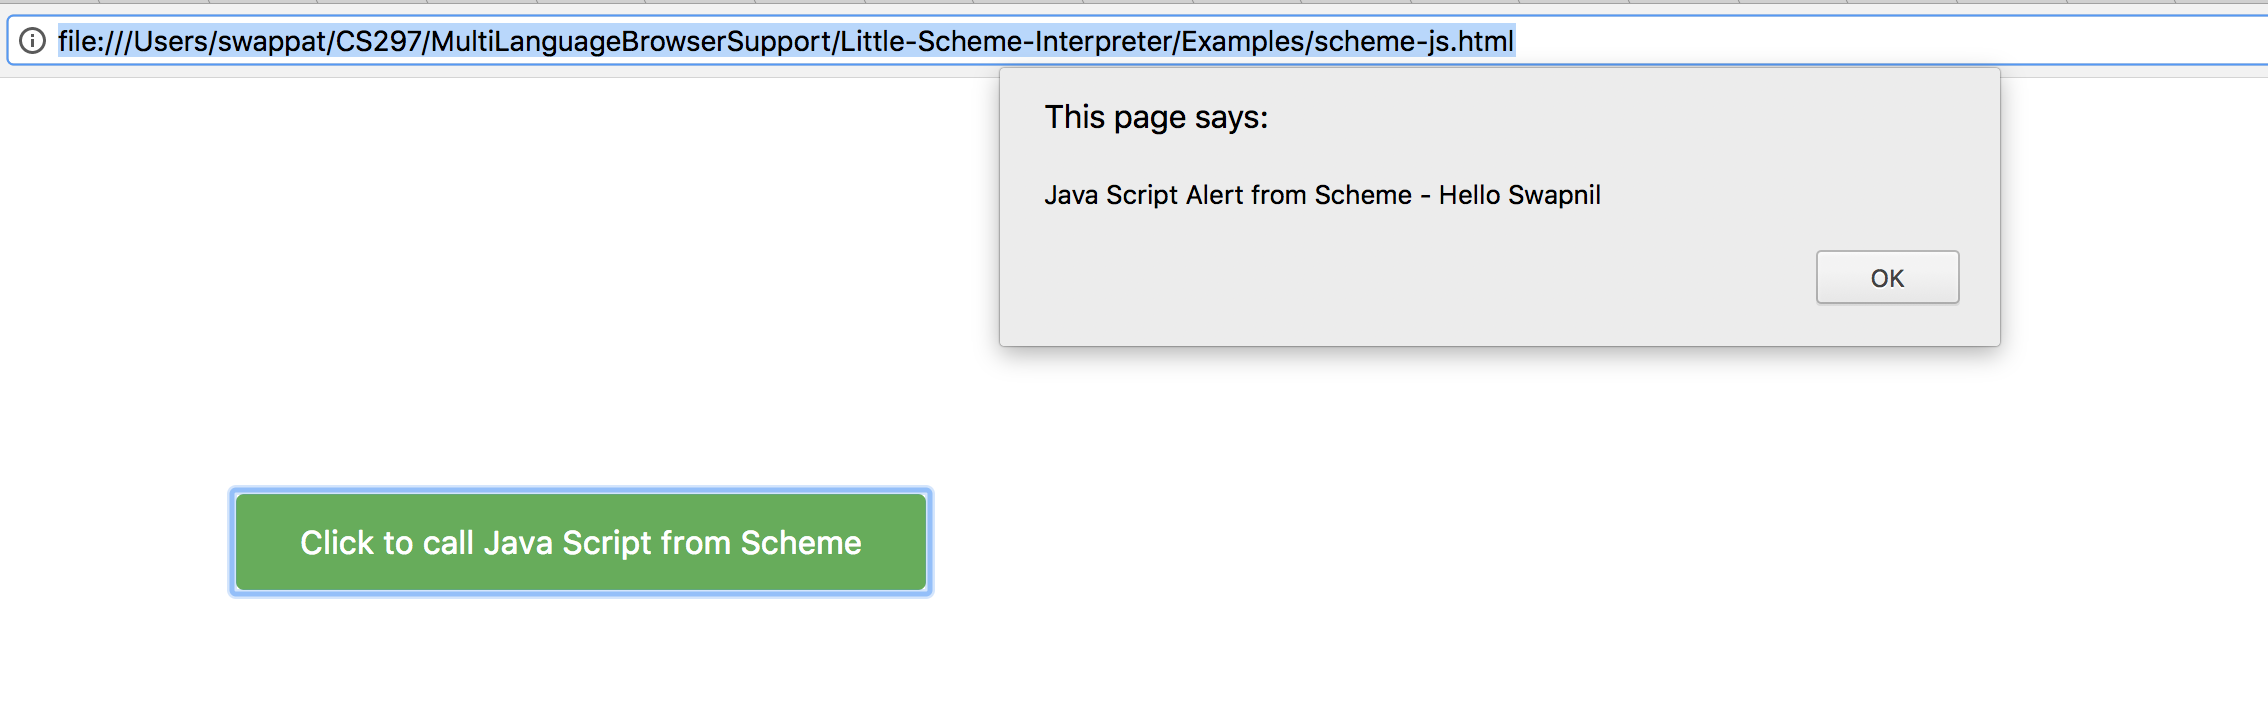
\includegraphics[width=\linewidth]{./images/scheme-js-interaction.png}
	\end{center}
	\caption{Calling JS from Scheme example: Output}
	\label{fig:scheme-js-interaction}
\end{figure}


\section{Calling Scheme from JS}

Similar to calling JavaScript code from the Scheme, we can also execute the Scheme code from JavaScript. The web page gets the instance of our Scheme interpreter by calling evaluate method on that instance. JavaScript can execute Scheme code as shown in Figure \ref{fig:js-scheme-interaction}. 


\begin{figure}[H]
	\begin{lstlisting}
	
  <input type=``button'' onclick=``callScheme()'' 
  id=``call'' value=``Execute Scheme Code 
  from Java Script'' />

  <script>
  function callScheme()
  {
   var sayHello = scheme.evaluate(``(lambda (msg)  
   (alert msg) )'');
   sayHello(``Calling Scheme method from JavaScript!!!!!'');
  }
</script>
</html>
	\end{lstlisting}
	\caption{Calling Scheme from JS}
	\label{fig:js-scheme-interaction}
\end{figure}



In the code shown in Figure \ref{fig:js-scheme-interaction}, we are evaluating function written in the Scheme and calling it from JavaScript. ``scheme.evaluate" function executes the Scheme code. In this case, we are storing Scheme lambda function in variable called ``sayHello'' and calling it with parameters from JavaScript, as shown in Figure \ref{fig:js-scheme-interaction}

\begin{figure}[H]
	\begin{center}
		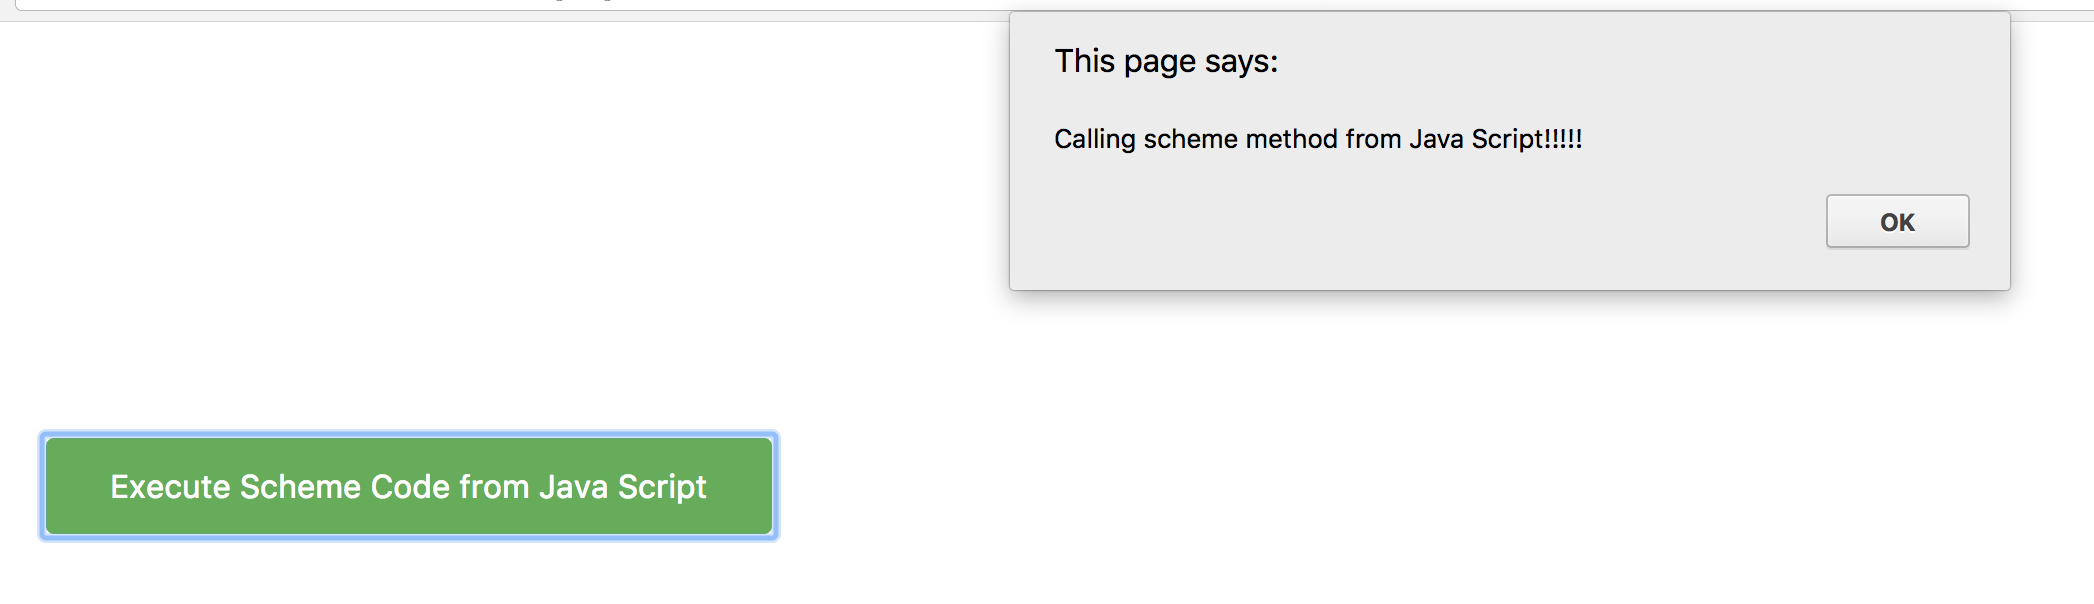
\includegraphics[width=\linewidth]{./images/js-scheme-interaction.png}
	\end{center}
	\caption{Calling Scheme from JS: Output}
	\label{fig:js-scheme-interaction}
\end{figure}


\section{Calling JS from  Lua}

Lua interacts with the JavaScript using eval function on the JavaScript global object. Code snippet in  Figure \ref{fig:js-lua-interaction} shows how to write the Lua code in the Lua script and shows how to access JavaScript code from Lua script.


\begin{figure}[H]
	\begin{lstlisting}
	<script src=``lua.vm.js''></script>
	<script type=``text/lua''>
	-- global object in JS is the window
	 local window = js.global 
	
	 -- Lua executing Java Script code
	 window:eval(`function sayHello (message)' ..
	  `{ alert(message); }' ..
	  `sayHello(``Hello from Java Script calling from Lua'');'
	 ) 
	
	 -- Alert from Lua
	 window:alert(``hello from lua!'')
	
	
	 -- Accessing DOM APIS from Lua
	 local document = js.global.document
	 print(``This window has title `'' .. document.title .. ``''')
	
	 -- function
	 function printWindowSize ()
	  local screen = js.global.screen
	  print(``you haz '' .. (screen.width*screen.height) .. 
	  `` pixels'')
	 end
	
	 printWindowSize()
	</script>
	\end{lstlisting}
	\caption{Calling JS from Lua}
	\label{fig:js-lua-interaction}
\end{figure}


In the code snippet shown in Figure \ref{fig:js-lua-interaction} the Lua environment is creating JavaScript function called ``sayHello'' and it is calling it using eval function on the JavaScript global object. Output of the code snippet is shown in Figures \ref{fig:alert-from-javascript-eval} - \ref{fig:printing-document-title}.

\begin{figure}[H]
	\begin{center}
		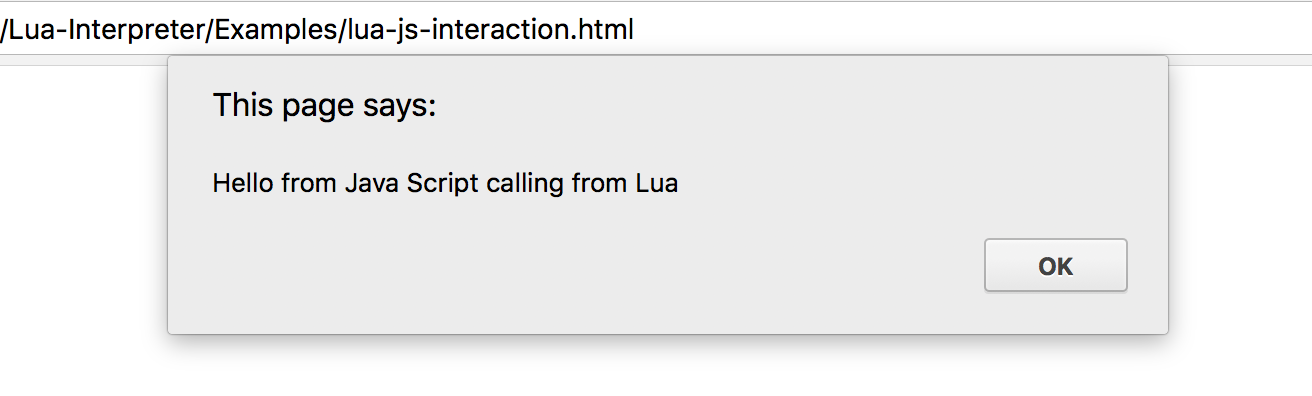
\includegraphics[width=\linewidth]{./images/alert-from-javascript-eval.png}
	\end{center}
	\caption{Executing JS from Lua Script: Output}
	\label{fig:alert-from-javascript-eval}
\end{figure}

\begin{figure}[H]
	\begin{center}
		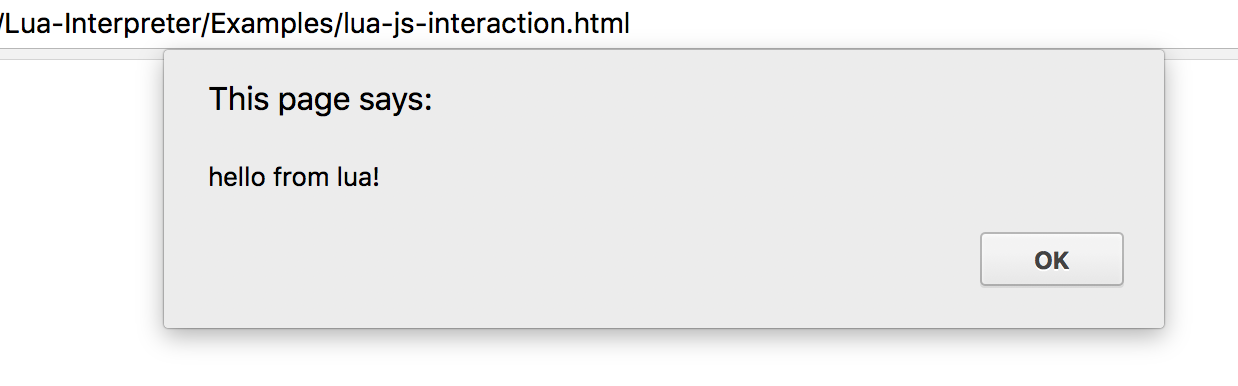
\includegraphics[width=\linewidth]{./images/alert-from-lua.png}
	\end{center}
	\caption{Alert from Lua : Output}
	\label{fig:alert-from-lua}
\end{figure}

\begin{figure}[H]
	\begin{center}
		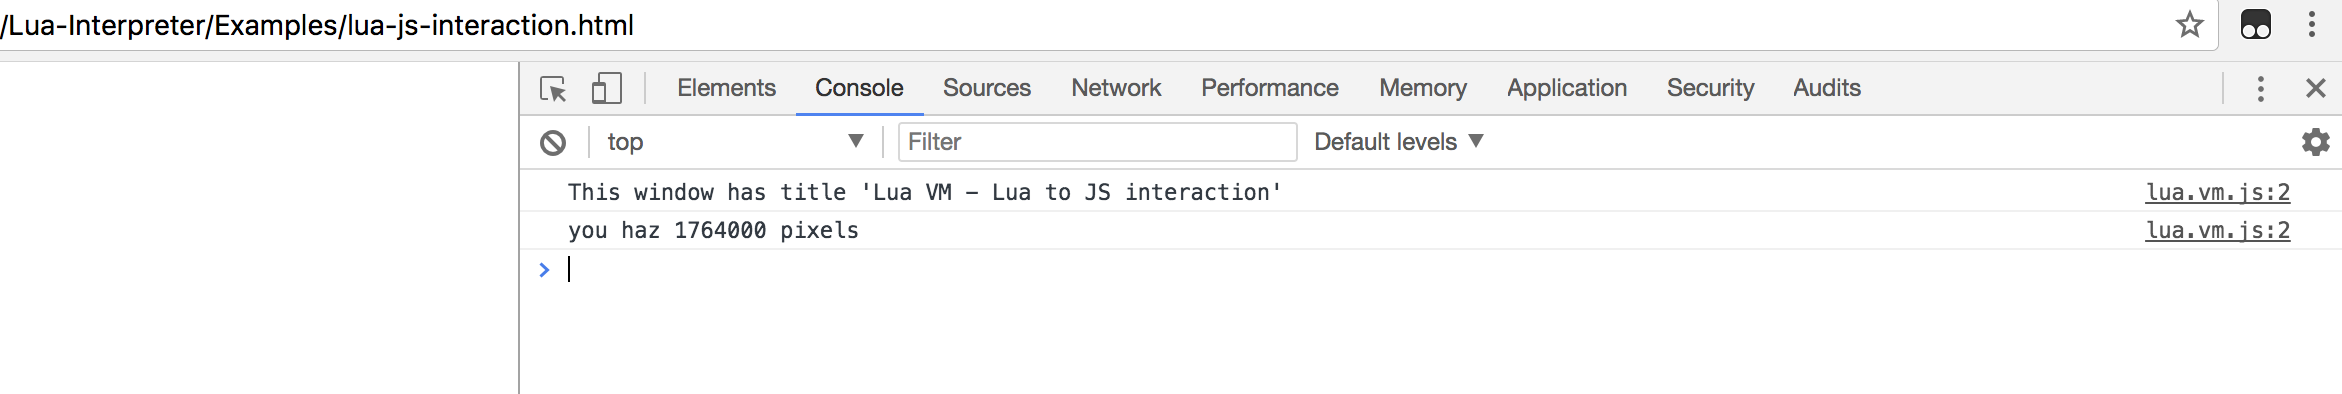
\includegraphics[width=\linewidth]{./images/printing-document-title.png}
	\end{center}
	\caption{Accessing DOM from Lua: Output}
	\label{fig:printing-document-title}
\end{figure}

\section{Calling Lua from JS}

The JavaScript interacts with the Lua using the ``L.execute'' function provided by the Lua VM. It accepts any Lua code as a string and executes it in JavaScript environment by calling the function, as shown in Figure \ref{fig:callingluafromjs}. 


\begin{figure}[H]
	\begin{lstlisting}[frame=single, style=base]

	<script src=``lua.vm.js''></script>
	<script>
	 function sayHello(message) {
	  console.log(message);
	 }
	
	 L.execute( // Lua Function Declaration
	  ``function printName (recipient) '' +
	  ``print(`Hello, '..recipient)'' +
	  ``end '' +
	
	  // Call to Lua Function
	  ``printName(`CS298 Project') '' +
	
	 // Calling Java Script function from Lua 
	 ``js.global:sayHello(`Hello to JS function')'' +
	
	 // Alert from Lua 
	 ``js.global:alert(`Hello from Lua') ''
	); 

	</script>
	\end{lstlisting}
	\caption{Calling Lua from JS}
	\label{fig:callingluafromjs}
\end{figure}


The code snippet shown in Figure \ref{fig:callingluafromjs} calls the Lua code from JavaScript environment. It creates Lua function called ``printName'', which prints the message on the console. This function is called with a parameter ``CS 298 Project". It also calls JavaScript function called ``sayHello'' from the Lua code. And similarly, it alerts ``Hello from Lua" message using Scheme alert function. Output of the above code snippet is shown in Figure \ref{fig:js-to-lua-interaction}.

\begin{figure}[H]
	\begin{center}
		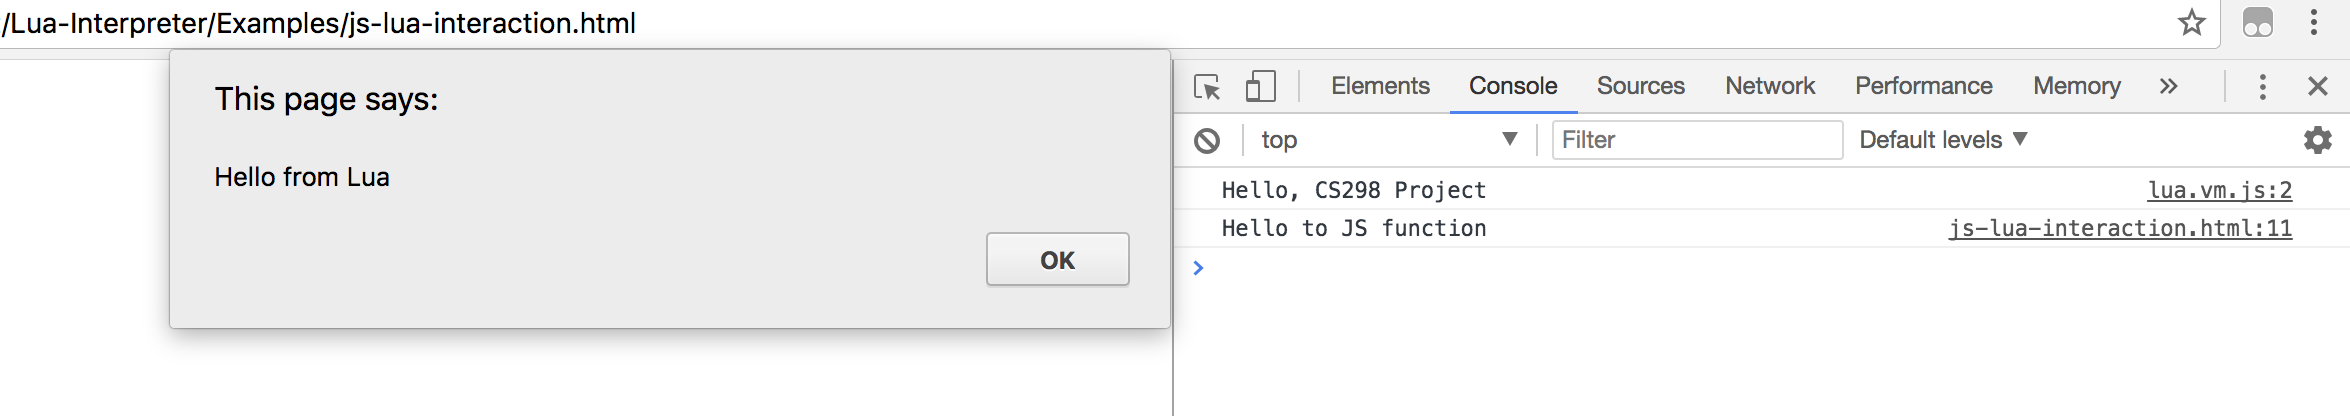
\includegraphics[width=\linewidth]{./images/js-to-lua-interaction.png}
	\end{center}
	\caption{Calling Lua from JS: Output}
	\label{fig:js-to-lua-interaction}
\end{figure}


